\begin{figure}[H]
    \centering
    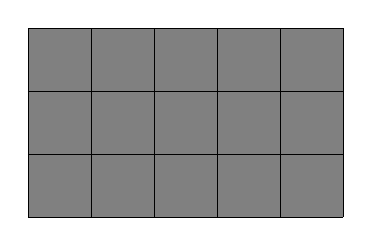
\begin{tikzpicture}[scale=0.8]
        \foreach \x in {0,...,4} {
            \foreach \y in {0,...,2} {
                \fill[gray] (\x,\y) rectangle ++(1,1);
            }
        }
        \draw[step=1cm,ultra thin,black] (0,0) grid (5,3);
    \end{tikzpicture}
    \caption{\centering Cała plansza stanowi ściany.}
    \label{fig:dfs_gen_step_1}
\end{figure}